\section{Identifying Trends}  \label{sec:features}

\begin{figure}
    \centering
    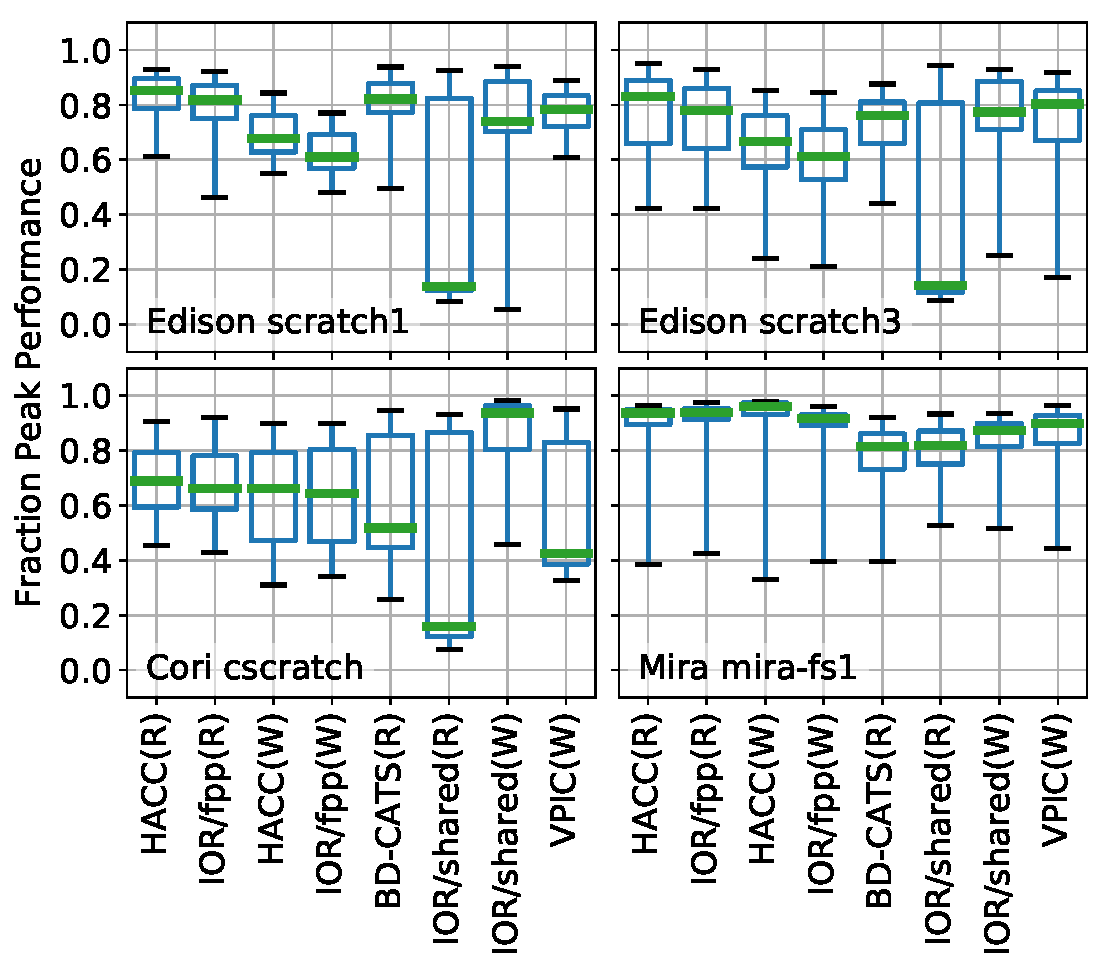
\includegraphics[width=0.9\columnwidth]{summary-boxplots}
    \vspace{-.15in}
    \caption{I/O performance grouped by I/O motifs and read(R)/write(W) mode.  Whiskers represent the 5th and 95th percentiles.}
    \label{fig:summary-boxplots}
\end{figure}

\begin{figure*}
    \centering
    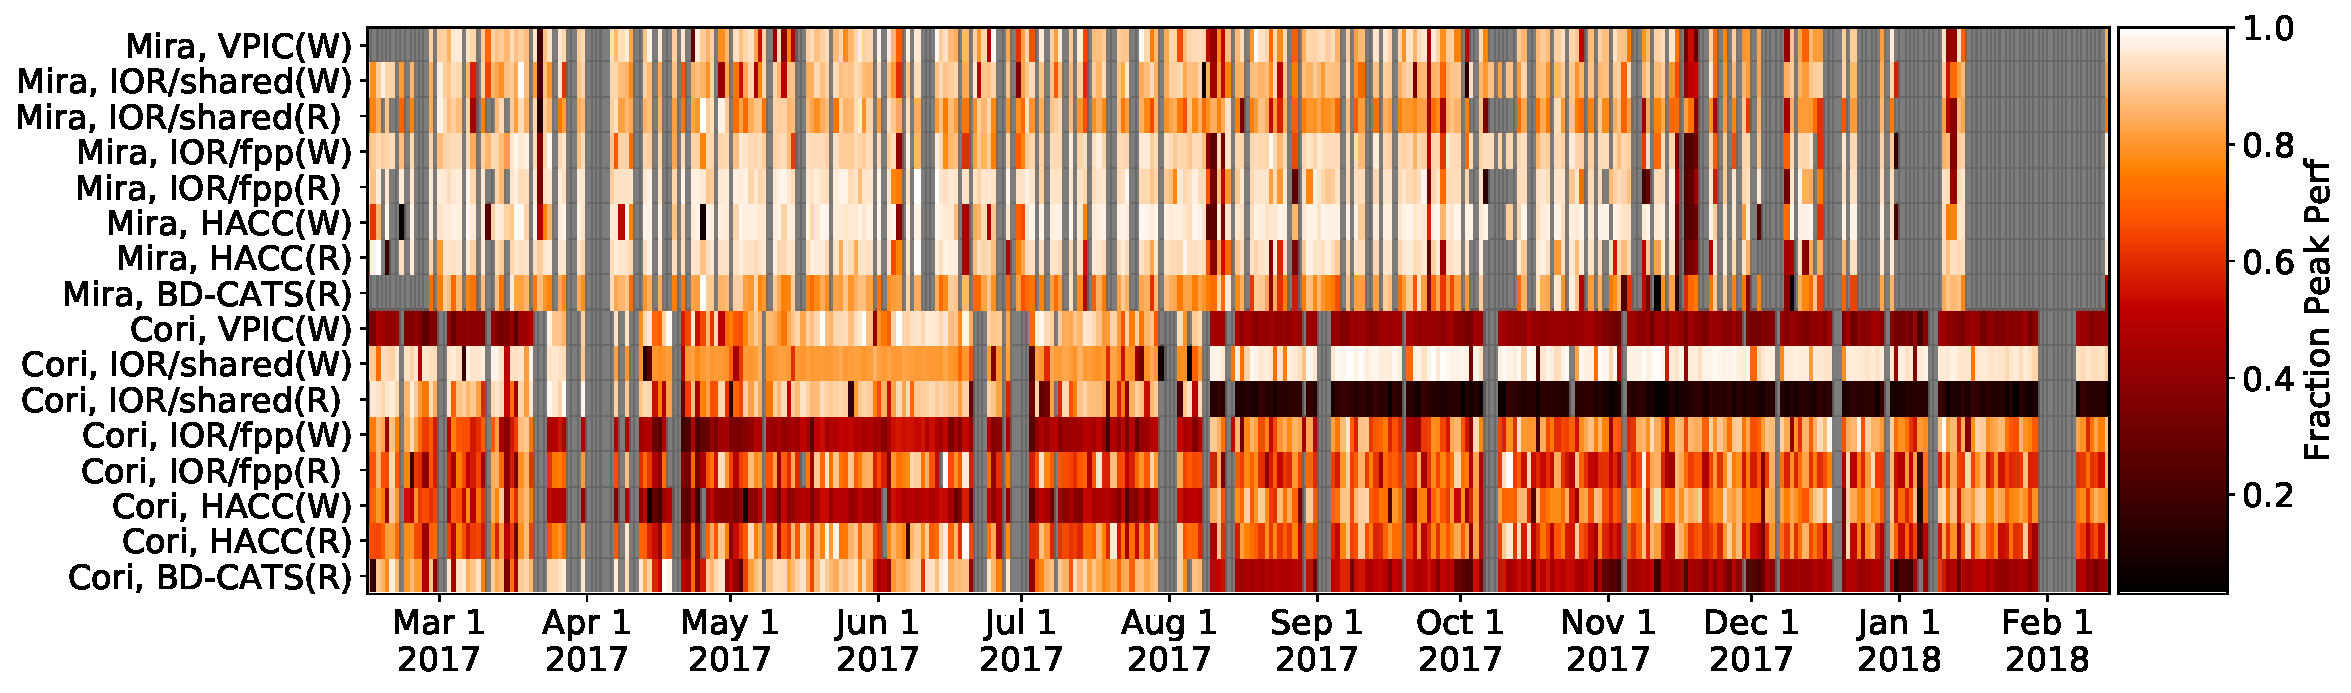
\includegraphics[width=0.90\linewidth]{summary-heatmap}
    \vspace{-.2in}
    \caption{Performance of daily probes normalized to the peak observed performance for each probe type (I/O motif and read/write mode combination) on the specified system.  The y-axis labels show combinations of system, I/O motif, and mode (Read/Write).  Grey represents days on which no observations were made.  The two regions highlighted in green boxes are expanded upon in Figure \ref{fig:regions-heatmap}.}
    \label{fig:summary-heatmap}
\end{figure*}

\begin{figure}
    \centering
    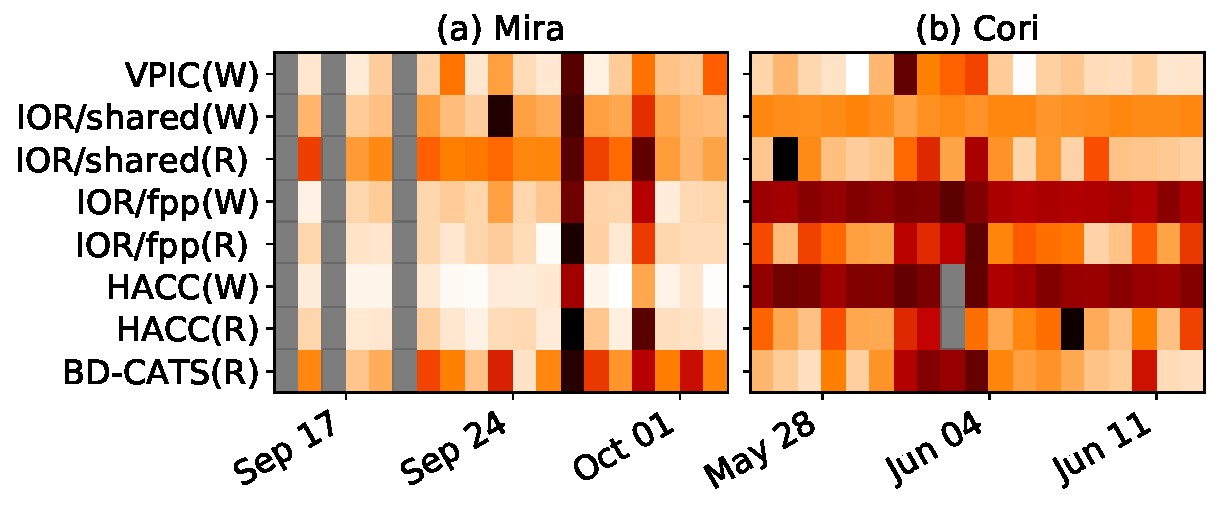
\includegraphics[width=0.90\linewidth]{regions-heatmap}
    \vspace{-.2in}
    \caption{Examples of structure in the fraction of peak performance observations.  Color scale is the same as that in Figure \ref{fig:summary-heatmap}.  In (a), the vertical band on Sept 26 corresponds to a transient system-wide degradation on \mira.  The horizontal bands for the IOR file-per-process write workload (IOR/fpp(W)) and HACC write workload (HACC(W)) in (b) show a sustained performance problem for file-per-process write workloads on \cori.}
    \label{fig:regions-heatmap}
\end{figure}




\subsection{Dataset overview} \label{sec:features/summary}

% \TODO{Things that are important here: behavior over time, grouping data sources in a way that helps understand scope, focusing on fundamental \emph{changes} in performance rather than steady state, everything in one view.}

Absolute I/O performance is influenced by many factors, most notably (a)
application I/O pattern, (b) read/write ratio, and (c) I/O system
architecture~\cite{Lockwood2017, Xie2012}.  This makes it difficult to
reason about performance variation across benchmarks or across platforms,
because each combination is capable of a different baseline performance
level.  We
address this problem by normalizing the
performance of each of the 11,986 observations in terms of its
\emph{fraction of peak performance}.
The fraction of peak performance is defined as the absolute performance (in
bytes/sec) of an observation divided by the maximum absolute performance
observed across all jobs with a common (a), (b), and (c) above.  This
approach allows us to focus on variability for different classes of I/O
workloads rather than their relative performance.

The distribution of the fraction of peak performance measurements for four
of the five systems tested is shown in Fig. \ref{fig:summary-boxplots}.
This figure illustrates that the performance of active I/O performance
probes on production file systems is highly dynamic over the course of a
year.  It does not provide any insight into the temporal nature of the
performance fluctuations, however.

Figure~\ref{fig:summary-heatmap} visualizes the same data in the form of a
heatmap over time.  This shows that performance variation is not randomly
distributed over the year; this is a key characteristic that is not captured by
time-independent performance distributions.
Several archetypical forms of correlated performance degradation observed in Fig. \ref{fig:summary-heatmap} are highlighted in Fig. \ref{fig:regions-heatmap} and fall into three broad categories of variation:

\begin{enumerate}[leftmargin=*]
\item Dark vertical bands, exemplified in the \mira data in Fig. \ref{fig:regions-heatmap}a, represent transient system-wide issues that resulted in a uniform loss of performance for all probes executed that day.
\item Dark horizontal bands, shown in the \cori data in Fig. \ref{fig:regions-heatmap}b, indicate a long-term degradation in performance that disproportionately affects a specific I/O motif.
\item Isolated dark blocks represent individual probes where performance was poor for a very short period of time within a day.
\end{enumerate}

% - Baseline performance and variability are not constant over time.  Predictive models must therefore adapt over time as well.
The preponderance of these time-dependent phenomena underscore the observation that \textbf{baseline I/O performance and variability are not constant over time}, and
what may qualify as abnormally poor performance during one period of time may be the baseline performance expectation during another.

This has implications for both HPC facility operators and users.  For
facility operators, it indicates that performance anomalies and their root
causes should not be assessed in isolation. By integrating broader spatial and
temporal context into the analysis, facility operators can more accurately
discriminate between application problems and environmental factors.
% From Phil: In the prose we can site several predictive model papers (Bing Xie's papers, Sandeep's papers, and others) and point out that the implication is that these models aren't just "set it and forget it."  Not knocking them or even saying they can't do it, but just pointing out it's not covered yet.
For users and application developers, it follows that the accuracy of parameterized I/O performance models~\cite{Xie2012,Madireddy2017} will degrade unless they are reparameterized as the I/O subsystem they model evolves.
Both of these cases justify the need for a systematic approach for identifying different regions of I/O performance to differentiate long-term factors and phenomena from short-term transients.

\subsection{Time-dependent analysis} \label{sec:features/timedependent}

Section~\ref{sec:features/summary} clearly illustrates the presence of
time-varying behavior, but quantitative methods are needed to extract 
actionable insight from these observations.  The main challenge that these
methods face is differentating performance trends from individual short-term
fluctuations in timeseries data.
This problem is not unique to I/O performance or even computer science,
however.  Notably, financial market technical analysis techniques are
routinely used for a similar purpose: attenuating day-to-day volatility in
the price of assets and identifying price movement
trends~\cite{james1968monthly,gunasekarage2001profitability}.  

The most straightforward initial technique to apply from this domain is
the use of Simple Moving Averages (SMAs) over the performance observations.
Given a time window of width $w$, the SMA for performance at time $t$ is the arithmetic mean of the fraction peak performance over ${-0.5w <= t < +0.5w}$.
When chosen to be sufficiently short (${w_{short} \sim O(\textup{days})}$),
the resulting $\textup{SMA}_{short}$ provides a rapid visual means to
identify performance degradation or recovery that lasts for
$O(\textup{days})$.  Multiple SMAs can be plotted simultaneously over the
same data set to differentiate short and long term trends and identify key
crossover points. 

\begin{figure}[t]
    \centering
    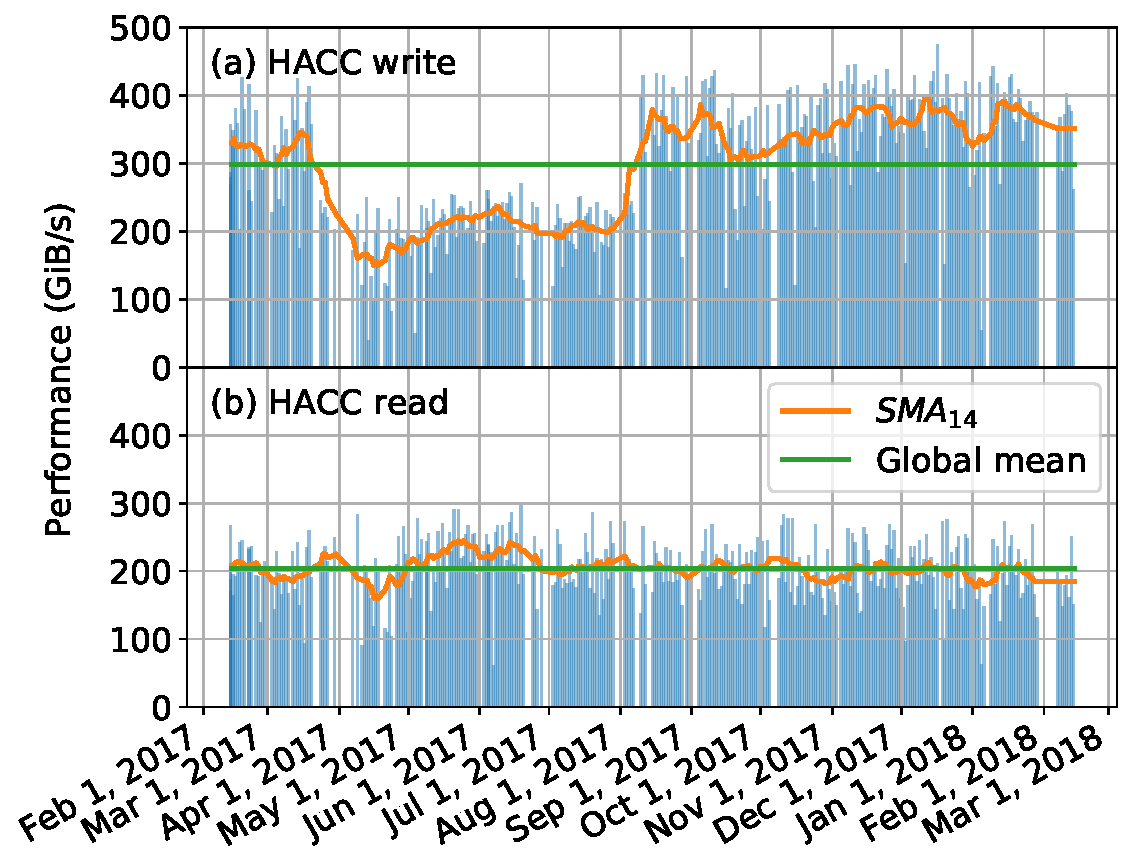
\includegraphics[width=1.0\columnwidth]{longterm-cscratch-hacc}
    \vspace{-.35in}
    \caption{Performance evolution of HACC file-per-process workload on \cori.  Red line is the overall mean (298 GiB/sec write, 204 GiB/sec read) and blue bars are raw performance measurements.}
    \label{fig:timeseries-baseline}
    % source: sc18_segments.ipynb
\end{figure}


An example of an SMA ($w_{short}$ = two weeks) applied to the performance data collected from HACC tests run on \cori is shown in Fig. \ref{fig:timeseries-baseline}.
When contrasted with a time-independent summary statistic such as the overall mean performance of the entire year, the SMA clearly identifies the long period of degraded HACC write performance on \cori that was qualitatively shown in the bottom half of Fig. \ref{fig:summary-heatmap}.
The points at which the SMA rise above or below the global mean performance also provide quantitative measurements of the region of time when an underlying issue manifested;
in Fig. \ref{fig:timeseries-baseline}, these \emph{crossover points} fall on March 24 and August 10.
Cross-referencing these dates with the service history of \cori retrospectively revealed that the beginning and end of this long-term region of divergent performance coincided with major system software upgrades that also happened on March 24 and August 10.

Curiously, the performance of HACC read workload (Figure \ref{fig:timeseries-baseline}b) was unaffected during this time, demonstrating that not all workloads are affected by long-term variation equally.
This asymmetry, in combination with the bounding dates of this divergent region, allowed us to trace this specific issue to unintentional behavior introduced (and later fixed) in the Lustre software running on \cori between the system upgrades.
Although this particular case of long-term performance divergence was caused by an unexpected bug in system software, the reality of most production storage systems is that they are regularly patched and upgraded.
At minimum, the security requirements of the centers which run them drive system updates, and as exemplified by the widely publicized Spectre and Meltdown patches, such updates can have non-trivial effects on certain types of I/O.
Thus, \textbf{administrative activities such as maintenance patches and
software updates are a significant source of time-dependent, long term performance
variation.}  This must be accounted for in both retrospective performance
analysis and forward looking performance modeling parameterization.  The
ramifications I/O research practitioners is that \textbf{holistic I/O monitoring
should incorporate environmental provinence
information, such as kernel, operating system, and file
system version, to aid in correlation.}

\subsection{Regions of interest} \label{sec:features/partitioning}

We can generalize the analysis technique from
Section~\ref{sec:features/timedependent} 
by superimposing a second SMA ($\textup{SMA}_{long}$) with a longer window (${w_{long} \sim O(\textup{weeks})}$) on top of $\textup{SMA}_{short}$ (which captures variations ${O(\textup{days})}$).
Doing so allows us to examine short-term performance variations (e.g., a
period of sustained bandwidth contention) in the context of longer-term
trends (e.g., in the presence of a file system software regression).  Once a
region of interest has been defined, we can then constrain more detailed
analysis techniques to that region to determine its cause.
The points at which $\textup{SMA}_{short}$ intersects $\textup{SMA}_{long}$, termed \emph{crossover points}, conveniently establish the boundaries of regions where short-term performance has diverged from longer-term performance and anomalous performance is prevailing.
We therefore introduce the notion of \emph{divergence regions} which are the periods of time bounded by two crossover points and capture correlated performance.
Fig. \ref{fig:mira-regions-overview} depicts how these concepts are applied in a subset of the data collected from \mira.

For the remainder of this study, we apply the concept of \emph{divergence regions}, bounded by the crossovers between $\textup{SMA}_{short}$ and $\textup{SMA}_{long}$, to systematically identify and characterize periods in time where anomalous performance was observed by the active I/O performance probes running across all of the test systems.
We define $\textup{SMA}_{short}$ to have ${w_{short} = \textup{two weeks}}$ as in \ref{sec:features/timedependent} and $\textup{SMA}_{long}$ to have ${w_{long} = \textup{seven weeks}}$.
$w$ was chosen to be a multiple of seven days to align with one
week and ensure that weekends and weekdays were equally represented in both SMA
calculations. $w_{long}$ was set to seven weeks to span multiple $w_{short}$
regions and at least one month boundary.  In our experience, the analysis
presented in this work was insensitive to changes of $\pm 1 \textup{ week}$.

In general we find that \textbf{financial market technical
analysis techniques can be adapted to
timeseries I/O performance data to attenuate noise and identify underlying trends.}
In the context of financial markets, SMAs (and other more
sophisticated related techniques) are used for predictive purposes to time
the execution of market trades.  In this context we are not applying them to
the task of predicting performance, but rather to identify regions of
interest in behavior that has already been recorded.

\begin{figure}
    \centering
    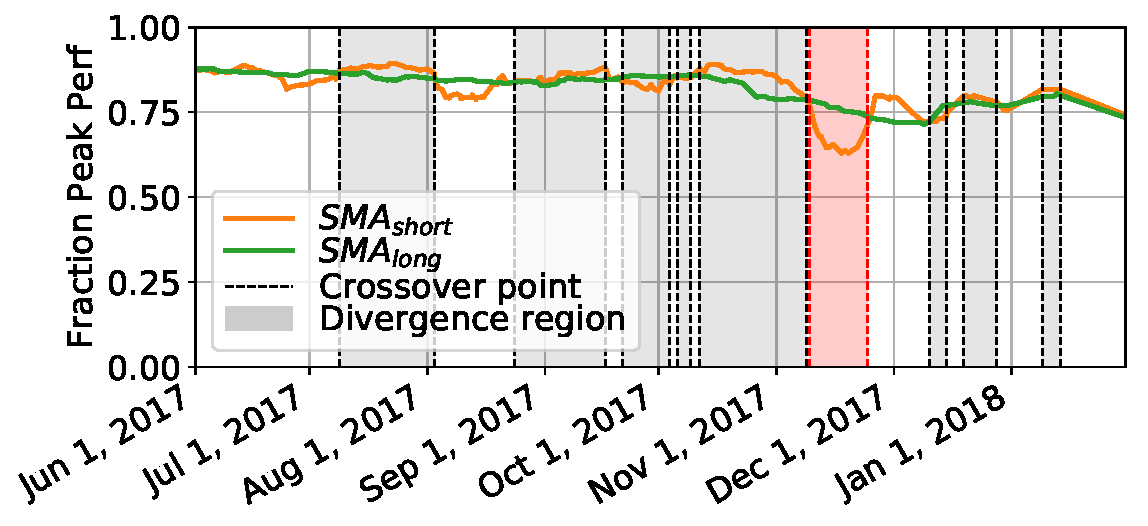
\includegraphics[width=1.0\columnwidth]{mira-regions-overview}
    \vspace{-.15in}
    \caption{Schematic depicting the relationship between SMAs, crossover points, and divergence regions on \mira.
    Both white and grey regions between crossovers are divergence regions, but only a subset of divergence regions are shaded for clarity.
    The significance of the divergence region highlighted in red is discussed in Section \ref{sec:results/correlate-mira}.}
    \label{fig:mira-regions-overview}
    % source: sc18_region-correlation.ipynb
\end{figure}
